\documentclass[1p]{elsarticle_modified}
%\bibliographystyle{elsarticle-num}

%\usepackage[colorlinks]{hyperref}
%\usepackage{abbrmath_seonhwa} %\Abb, \Ascr, \Acal ,\Abf, \Afrak
\usepackage{amsfonts}
\usepackage{amssymb}
\usepackage{amsmath}
\usepackage{amsthm}
\usepackage{scalefnt}
\usepackage{amsbsy}
\usepackage{kotex}
\usepackage{caption}
\usepackage{subfig}
\usepackage{color}
\usepackage{graphicx}
\usepackage{xcolor} %% white, black, red, green, blue, cyan, magenta, yellow
\usepackage{float}
\usepackage{setspace}
\usepackage{hyperref}

\usepackage{tikz}
\usetikzlibrary{arrows}

\usepackage{multirow}
\usepackage{array} % fixed length table
\usepackage{hhline}

%%%%%%%%%%%%%%%%%%%%%
\makeatletter
\renewcommand*\env@matrix[1][\arraystretch]{%
	\edef\arraystretch{#1}%
	\hskip -\arraycolsep
	\let\@ifnextchar\new@ifnextchar
	\array{*\c@MaxMatrixCols c}}
\makeatother %https://tex.stackexchange.com/questions/14071/how-can-i-increase-the-line-spacing-in-a-matrix
%%%%%%%%%%%%%%%

\usepackage[normalem]{ulem}

\newcommand{\msout}[1]{\ifmmode\text{\sout{\ensuremath{#1}}}\else\sout{#1}\fi}
%SOURCE: \msout is \stkout macro in https://tex.stackexchange.com/questions/20609/strikeout-in-math-mode

\newcommand{\cancel}[1]{
	\ifmmode
	{\color{red}\msout{#1}}
	\else
	{\color{red}\sout{#1}}
	\fi
}

\newcommand{\add}[1]{
	{\color{blue}\uwave{#1}}
}

\newcommand{\replace}[2]{
	\ifmmode
	{\color{red}\msout{#1}}{\color{blue}\uwave{#2}}
	\else
	{\color{red}\sout{#1}}{\color{blue}\uwave{#2}}
	\fi
}

\newcommand{\Sol}{\mathcal{S}} %segment
\newcommand{\D}{D} %diagram
\newcommand{\A}{\mathcal{A}} %arc


%%%%%%%%%%%%%%%%%%%%%%%%%%%%%5 test

\def\sl{\operatorname{\textup{SL}}(2,\Cbb)}
\def\psl{\operatorname{\textup{PSL}}(2,\Cbb)}
\def\quan{\mkern 1mu \triangleright \mkern 1mu}

\theoremstyle{definition}
\newtheorem{thm}{Theorem}[section]
\newtheorem{prop}[thm]{Proposition}
\newtheorem{lem}[thm]{Lemma}
\newtheorem{ques}[thm]{Question}
\newtheorem{cor}[thm]{Corollary}
\newtheorem{defn}[thm]{Definition}
\newtheorem{exam}[thm]{Example}
\newtheorem{rmk}[thm]{Remark}
\newtheorem{alg}[thm]{Algorithm}

\newcommand{\I}{\sqrt{-1}}
\begin{document}

%\begin{frontmatter}
%
%\title{Boundary parabolic representations of knots up to 8 crossings}
%
%%% Group authors per affiliation:
%\author{Yunhi Cho} 
%\address{Department of Mathematics, University of Seoul, Seoul, Korea}
%\ead{yhcho@uos.ac.kr}
%
%
%\author{Seonhwa Kim} %\fnref{s_kim}}
%\address{Center for Geometry and Physics, Institute for Basic Science, Pohang, 37673, Korea}
%\ead{ryeona17@ibs.re.kr}
%
%\author{Hyuk Kim}
%\address{Department of Mathematical Sciences, Seoul National University, Seoul 08826, Korea}
%\ead{hyukkim@snu.ac.kr}
%
%\author{Seokbeom Yoon}
%\address{Department of Mathematical Sciences, Seoul National University, Seoul, 08826,  Korea}
%\ead{sbyoon15@snu.ac.kr}
%
%\begin{abstract}
%We find all boundary parabolic representation of knots up to 8 crossings.
%
%\end{abstract}
%\begin{keyword}
%    \MSC[2010] 57M25 
%\end{keyword}
%
%\end{frontmatter}

%\linenumbers
%\tableofcontents
%
\newcommand\colored[1]{\textcolor{white}{\rule[-0.35ex]{0.8em}{1.4ex}}\kern-0.8em\color{red} #1}%
%\newcommand\colored[1]{\textcolor{white}{ #1}\kern-2.17ex	\textcolor{white}{ #1}\kern-1.81ex	\textcolor{white}{ #1}\kern-2.15ex\color{red}#1	}

{\Large $\underline{12n_{0693}~(K12n_{0693})}$}

\setlength{\tabcolsep}{10pt}
\renewcommand{\arraystretch}{1.6}
\vspace{1cm}\begin{tabular}{m{100pt}>{\centering\arraybackslash}m{274pt}}
\multirow{5}{120pt}{
	\centering
	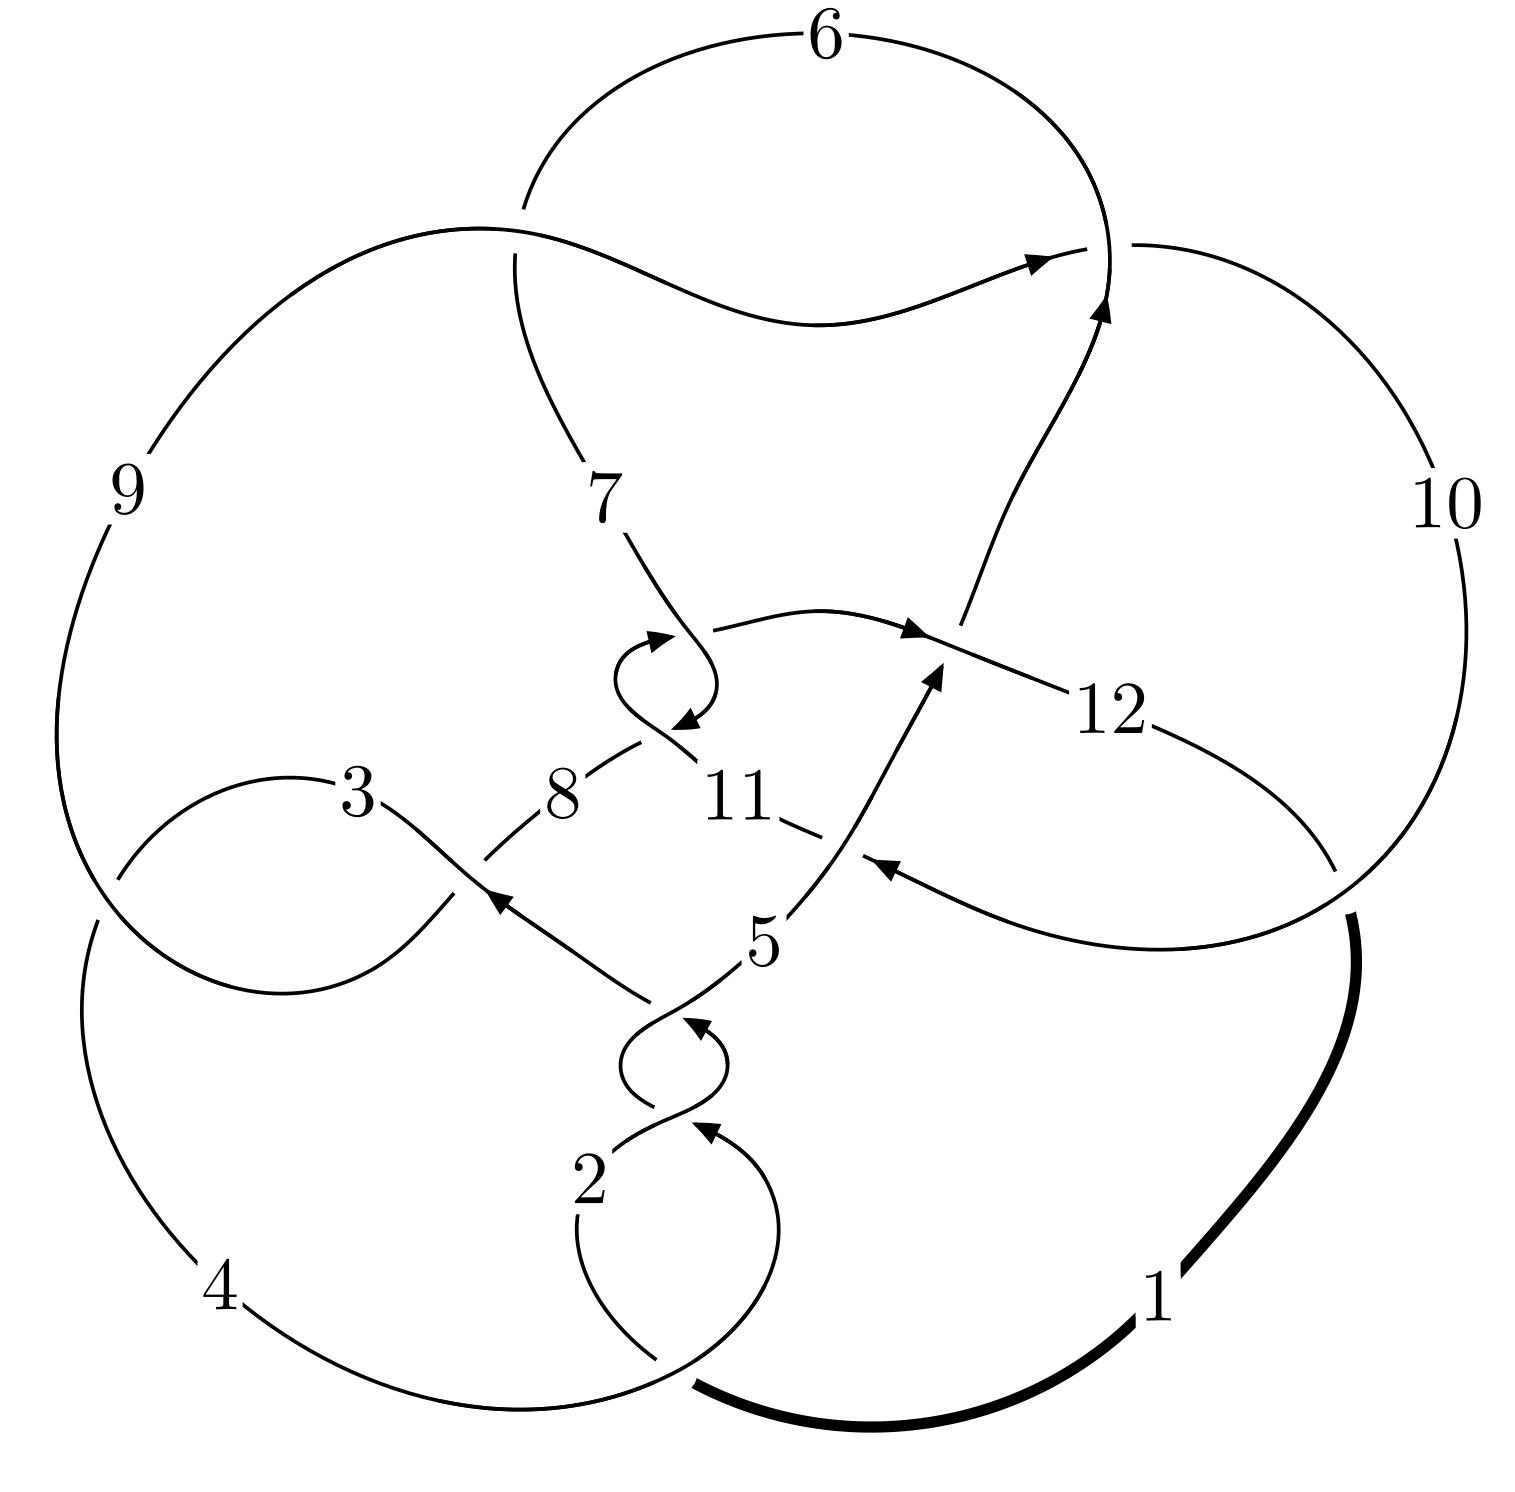
\includegraphics[width=112pt]{../../../GIT/diagram.site/Diagrams/png/2782_12n_0693.png}\\
\ \ \ A knot diagram\footnotemark}&
\allowdisplaybreaks
\textbf{Linearized knot diagam} \\
\cline{2-2}
 &
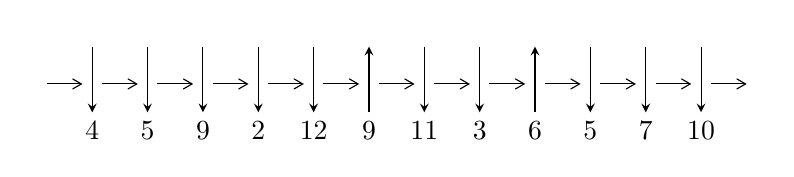
\begin{tikzpicture}[x=20pt, y=17pt]
	% nodes
	\node (C0) at (0, 0) {};
	\node (C1) at (1, 0) {};
	\node (C1U) at (1, +1) {};
	\node (C1D) at (1, -1) {4};

	\node (C2) at (2, 0) {};
	\node (C2U) at (2, +1) {};
	\node (C2D) at (2, -1) {5};

	\node (C3) at (3, 0) {};
	\node (C3U) at (3, +1) {};
	\node (C3D) at (3, -1) {9};

	\node (C4) at (4, 0) {};
	\node (C4U) at (4, +1) {};
	\node (C4D) at (4, -1) {2};

	\node (C5) at (5, 0) {};
	\node (C5U) at (5, +1) {};
	\node (C5D) at (5, -1) {12};

	\node (C6) at (6, 0) {};
	\node (C6U) at (6, +1) {};
	\node (C6D) at (6, -1) {9};

	\node (C7) at (7, 0) {};
	\node (C7U) at (7, +1) {};
	\node (C7D) at (7, -1) {11};

	\node (C8) at (8, 0) {};
	\node (C8U) at (8, +1) {};
	\node (C8D) at (8, -1) {3};

	\node (C9) at (9, 0) {};
	\node (C9U) at (9, +1) {};
	\node (C9D) at (9, -1) {6};

	\node (C10) at (10, 0) {};
	\node (C10U) at (10, +1) {};
	\node (C10D) at (10, -1) {5};

	\node (C11) at (11, 0) {};
	\node (C11U) at (11, +1) {};
	\node (C11D) at (11, -1) {7};

	\node (C12) at (12, 0) {};
	\node (C12U) at (12, +1) {};
	\node (C12D) at (12, -1) {10};
	\node (C13) at (13, 0) {};

	% arrows
	\draw[->,>={angle 60}]
	(C0) edge (C1) (C1) edge (C2) (C2) edge (C3) (C3) edge (C4) (C4) edge (C5) (C5) edge (C6) (C6) edge (C7) (C7) edge (C8) (C8) edge (C9) (C9) edge (C10) (C10) edge (C11) (C11) edge (C12) (C12) edge (C13) ;	\draw[->,>=stealth]
	(C1U) edge (C1D) (C2U) edge (C2D) (C3U) edge (C3D) (C4U) edge (C4D) (C5U) edge (C5D) (C6D) edge (C6U) (C7U) edge (C7D) (C8U) edge (C8D) (C9D) edge (C9U) (C10U) edge (C10D) (C11U) edge (C11D) (C12U) edge (C12D) ;
	\end{tikzpicture} \\
\hhline{~~} \\& 
\textbf{Solving Sequence} \\ \cline{2-2} 
 &
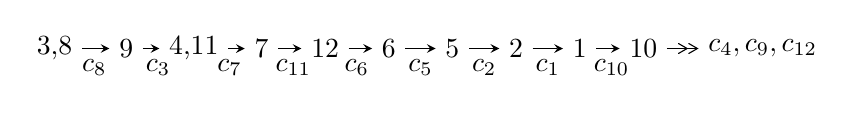
\begin{tikzpicture}[x=23pt, y=7pt]
	% node
	\node (A0) at (-1/8, 0) {3,8};
	\node (A1) at (1, 0) {9};
	\node (A2) at (33/16, 0) {4,11};
	\node (A3) at (25/8, 0) {7};
	\node (A4) at (33/8, 0) {12};
	\node (A5) at (41/8, 0) {6};
	\node (A6) at (49/8, 0) {5};
	\node (A7) at (57/8, 0) {2};
	\node (A8) at (65/8, 0) {1};
	\node (A9) at (73/8, 0) {10};
	\node (C1) at (1/2, -1) {$c_{8}$};
	\node (C2) at (3/2, -1) {$c_{3}$};
	\node (C3) at (21/8, -1) {$c_{7}$};
	\node (C4) at (29/8, -1) {$c_{11}$};
	\node (C5) at (37/8, -1) {$c_{6}$};
	\node (C6) at (45/8, -1) {$c_{5}$};
	\node (C7) at (53/8, -1) {$c_{2}$};
	\node (C8) at (61/8, -1) {$c_{1}$};
	\node (C9) at (69/8, -1) {$c_{10}$};
	\node (A10) at (11, 0) {$c_{4},c_{9},c_{12}$};

	% edge
	\draw[->,>=stealth]	
	(A0) edge (A1) (A1) edge (A2) (A2) edge (A3) (A3) edge (A4) (A4) edge (A5) (A5) edge (A6) (A6) edge (A7) (A7) edge (A8) (A8) edge (A9) ;
	\draw[->>,>={angle 60}]	
	(A9) edge (A10);
\end{tikzpicture} \\ 

\end{tabular} \\

\footnotetext{
The image of knot diagram is generated by the software ``\textbf{Draw programme}" developed by Andrew Bartholomew(\url{http://www.layer8.co.uk/maths/draw/index.htm\#Running-draw}), where we modified some parts for our purpose(\url{https://github.com/CATsTAILs/LinksPainter}).
}\phantom \\ \newline 
\centering \textbf{Ideals for irreducible components\footnotemark of $X_{\text{par}}$} 
 
\begin{align*}
I^u_{1}&=\langle 
-1.19530\times10^{101} u^{27}-5.30605\times10^{101} u^{26}+\cdots+2.74772\times10^{105} b+4.81437\times10^{105},\\
\phantom{I^u_{1}}&\phantom{= \langle  }-1.14694\times10^{104} u^{27}-5.23246\times10^{104} u^{26}+\cdots+2.69277\times10^{107} a+4.77354\times10^{108},\\
\phantom{I^u_{1}}&\phantom{= \langle  }u^{28}+4 u^{27}+\cdots-75264 u+25088\rangle \\
I^u_{2}&=\langle 
-168189 u^{12}+367074 u^{11}+\cdots+485 b-207077,\;-34213 u^{12}+74426 u^{11}+\cdots+97 a-40975,\\
\phantom{I^u_{2}}&\phantom{= \langle  }u^{13}-3 u^{12}-3 u^{11}+4 u^{10}+u^9+5 u^8+12 u^7-23 u^6-15 u^5+13 u^4+12 u^3- u^2-3 u-1\rangle \\
\\
I^v_{1}&=\langle 
a,\;-82026 v^8-2033115 v^7+\cdots+764761 b+1552510,\\
\phantom{I^v_{1}}&\phantom{= \langle  }7 v^9+3 v^8+2 v^7-14 v^6-23 v^5+33 v^4- v^3-8 v^2+v+1\rangle \\
\end{align*}
\raggedright * 3 irreducible components of $\dim_{\mathbb{C}}=0$, with total 50 representations.\\
\footnotetext{All coefficients of polynomials are rational numbers. But the coefficients are sometimes approximated in decimal forms when there is not enough margin.}
\newpage
\renewcommand{\arraystretch}{1}
\centering \section*{I. $I^u_{1}= \langle -1.20\times10^{101} u^{27}-5.31\times10^{101} u^{26}+\cdots+2.75\times10^{105} b+4.81\times10^{105},\;-1.15\times10^{104} u^{27}-5.23\times10^{104} u^{26}+\cdots+2.69\times10^{107} a+4.77\times10^{108},\;u^{28}+4 u^{27}+\cdots-75264 u+25088 \rangle$}
\flushleft \textbf{(i) Arc colorings}\\
\begin{tabular}{m{7pt} m{180pt} m{7pt} m{180pt} }
\flushright $a_{3}=$&$\begin{pmatrix}0\\u\end{pmatrix}$ \\
\flushright $a_{8}=$&$\begin{pmatrix}1\\0\end{pmatrix}$ \\
\flushright $a_{9}=$&$\begin{pmatrix}1\\u^2\end{pmatrix}$ \\
\flushright $a_{4}=$&$\begin{pmatrix}- u\\- u^3+u\end{pmatrix}$ \\
\flushright $a_{11}=$&$\begin{pmatrix}0.000425935 u^{27}+0.00194315 u^{26}+\cdots+23.7900 u-17.7273\\0.0000435014 u^{27}+0.000193107 u^{26}+\cdots+1.17208 u-1.75213\end{pmatrix}$ \\
\flushright $a_{7}=$&$\begin{pmatrix}0.000282338 u^{27}+0.00130937 u^{26}+\cdots+17.6311 u-10.2877\\0.0000612204 u^{27}+0.000273967 u^{26}+\cdots+5.23614 u-2.64624\end{pmatrix}$ \\
\flushright $a_{12}=$&$\begin{pmatrix}0.000456925 u^{27}+0.00211671 u^{26}+\cdots+25.6324 u-17.7624\\0.0000693492 u^{27}+0.000324215 u^{26}+\cdots+2.03194 u-2.70300\end{pmatrix}$ \\
\flushright $a_{6}=$&$\begin{pmatrix}0.000335467 u^{27}+0.00156198 u^{26}+\cdots+18.8607 u-12.1578\\0.0000866890 u^{27}+0.000392041 u^{26}+\cdots+6.92109 u-3.65218\end{pmatrix}$ \\
\flushright $a_{5}=$&$\begin{pmatrix}0.0000436460 u^{27}+0.000197226 u^{26}+\cdots+1.36979 u-2.04087\\0.0000155704 u^{27}+0.0000694627 u^{26}+\cdots+1.84303 u-0.799131\end{pmatrix}$ \\
\flushright $a_{2}=$&$\begin{pmatrix}-0.0000475456 u^{27}-0.000214384 u^{26}+\cdots-2.60369 u+2.27196\\-8.68541\times10^{-6} u^{27}-0.0000387931 u^{26}+\cdots+0.605212 u+0.376080\end{pmatrix}$ \\
\flushright $a_{1}=$&$\begin{pmatrix}-0.0000592164 u^{27}-0.000266688 u^{26}+\cdots-3.21282 u+2.84000\\5.14630\times10^{-7} u^{27}+3.68556\times10^{-6} u^{26}+\cdots+1.08406 u-0.0509325\end{pmatrix}$ \\
\flushright $a_{10}=$&$\begin{pmatrix}0.000450336 u^{27}+0.00204929 u^{26}+\cdots+25.1559 u-19.3277\\0.0000492022 u^{27}+0.000219246 u^{26}+\cdots+1.32187 u-1.74134\end{pmatrix}$\\&\end{tabular}
\flushleft \textbf{(ii) Obstruction class $= -1$}\\~\\
\flushleft \textbf{(iii) Cusp Shapes $= -0.000152878 u^{27}-0.000780946 u^{26}+\cdots-9.76931 u-4.69330$}\\~\\
\newpage\renewcommand{\arraystretch}{1}
\flushleft \textbf{(iv) u-Polynomials at the component}\newline \\
\begin{tabular}{m{50pt}|m{274pt}}
Crossings & \hspace{64pt}u-Polynomials at each crossing \\
\hline $$\begin{aligned}c_{1},c_{2},c_{4}\end{aligned}$$&$\begin{aligned}
&u^{28}-16 u^{27}+\cdots+419 u-49
\end{aligned}$\\
\hline $$\begin{aligned}c_{3},c_{8}\end{aligned}$$&$\begin{aligned}
&u^{28}+4 u^{27}+\cdots-75264 u+25088
\end{aligned}$\\
\hline $$\begin{aligned}c_{5}\end{aligned}$$&$\begin{aligned}
&u^{28}-4 u^{27}+\cdots+9 u-9
\end{aligned}$\\
\hline $$\begin{aligned}c_{6},c_{9}\end{aligned}$$&$\begin{aligned}
&u^{28}+3 u^{27}+\cdots+300 u+59
\end{aligned}$\\
\hline $$\begin{aligned}c_{7},c_{11}\end{aligned}$$&$\begin{aligned}
&u^{28}+2 u^{27}+\cdots-1173 u-1219
\end{aligned}$\\
\hline $$\begin{aligned}c_{10}\end{aligned}$$&$\begin{aligned}
&u^{28}- u^{27}+\cdots-246402 u-218849
\end{aligned}$\\
\hline $$\begin{aligned}c_{12}\end{aligned}$$&$\begin{aligned}
&u^{28}- u^{27}+\cdots+26513 u+36713
\end{aligned}$\\
\hline
\end{tabular}\\~\\
\newpage\renewcommand{\arraystretch}{1}
\flushleft \textbf{(v) Riley Polynomials at the component}\newline \\
\begin{tabular}{m{50pt}|m{274pt}}
Crossings & \hspace{64pt}Riley Polynomials at each crossing \\
\hline $$\begin{aligned}c_{1},c_{2},c_{4}\end{aligned}$$&$\begin{aligned}
&y^{28}-4 y^{27}+\cdots-168113 y+2401
\end{aligned}$\\
\hline $$\begin{aligned}c_{3},c_{8}\end{aligned}$$&$\begin{aligned}
&y^{28}+78 y^{27}+\cdots+603717632 y+629407744
\end{aligned}$\\
\hline $$\begin{aligned}c_{5}\end{aligned}$$&$\begin{aligned}
&y^{28}+2 y^{27}+\cdots-657 y+81
\end{aligned}$\\
\hline $$\begin{aligned}c_{6},c_{9}\end{aligned}$$&$\begin{aligned}
&y^{28}+y^{27}+\cdots-86696 y+3481
\end{aligned}$\\
\hline $$\begin{aligned}c_{7},c_{11}\end{aligned}$$&$\begin{aligned}
&y^{28}+42 y^{27}+\cdots+5986831 y+1485961
\end{aligned}$\\
\hline $$\begin{aligned}c_{10}\end{aligned}$$&$\begin{aligned}
&y^{28}+53 y^{27}+\cdots+367398468196 y+47894884801
\end{aligned}$\\
\hline $$\begin{aligned}c_{12}\end{aligned}$$&$\begin{aligned}
&y^{28}+29 y^{27}+\cdots-4800844229 y+1347844369
\end{aligned}$\\
\hline
\end{tabular}\\~\\
\newpage\flushleft \textbf{(vi) Complex Volumes and Cusp Shapes}
$$\begin{array}{c|c|c}  
\text{Solutions to }I^u_{1}& \I (\text{vol} + \sqrt{-1}CS) & \text{Cusp shape}\\
 \hline 
\begin{aligned}
u &= \phantom{-}0.661495 + 0.747398 I \\
a &= -1.101650 + 0.440671 I \\
b &= -0.236907 + 0.377211 I\end{aligned}
 & -2.93456 - 1.71766 I & -11.35116 + 2.24777 I \\ \hline\begin{aligned}
u &= \phantom{-}0.661495 - 0.747398 I \\
a &= -1.101650 - 0.440671 I \\
b &= -0.236907 - 0.377211 I\end{aligned}
 & -2.93456 + 1.71766 I & -11.35116 - 2.24777 I \\ \hline\begin{aligned}
u &= -0.893984 + 0.439919 I \\
a &= \phantom{-}1.294490 + 0.133923 I \\
b &= \phantom{-}0.543436 - 0.602243 I\end{aligned}
 & -0.665833 - 0.463592 I & -8.88124 - 0.80143 I \\ \hline\begin{aligned}
u &= -0.893984 - 0.439919 I \\
a &= \phantom{-}1.294490 - 0.133923 I \\
b &= \phantom{-}0.543436 + 0.602243 I\end{aligned}
 & -0.665833 + 0.463592 I & -8.88124 + 0.80143 I \\ \hline\begin{aligned}
u &= -0.060146 + 1.078200 I \\
a &= \phantom{-}0.399755 - 0.111241 I \\
b &= \phantom{-}0.264455 - 0.608981 I\end{aligned}
 & \phantom{-}1.30627 + 3.65816 I & \phantom{-}0.62607 - 9.21590 I \\ \hline\begin{aligned}
u &= -0.060146 - 1.078200 I \\
a &= \phantom{-}0.399755 + 0.111241 I \\
b &= \phantom{-}0.264455 + 0.608981 I\end{aligned}
 & \phantom{-}1.30627 - 3.65816 I & \phantom{-}0.62607 + 9.21590 I \\ \hline\begin{aligned}
u &= \phantom{-}1.083710 + 0.326182 I \\
a &= -0.046362 - 0.438180 I \\
b &= -0.577733 + 1.217650 I\end{aligned}
 & -5.85717 + 6.56767 I & -13.7398 - 3.9298 I \\ \hline\begin{aligned}
u &= \phantom{-}1.083710 - 0.326182 I \\
a &= -0.046362 + 0.438180 I \\
b &= -0.577733 - 1.217650 I\end{aligned}
 & -5.85717 - 6.56767 I & -13.7398 + 3.9298 I \\ \hline\begin{aligned}
u &= -0.775820 + 0.972482 I \\
a &= \phantom{-}0.054417 + 0.688396 I \\
b &= -0.727007 - 1.203150 I\end{aligned}
 & -5.97045 + 2.54425 I & -12.99283 - 2.62358 I \\ \hline\begin{aligned}
u &= -0.775820 - 0.972482 I \\
a &= \phantom{-}0.054417 - 0.688396 I \\
b &= -0.727007 + 1.203150 I\end{aligned}
 & -5.97045 - 2.54425 I & -12.99283 + 2.62358 I\\
 \hline 
 \end{array}$$\newpage$$\begin{array}{c|c|c}  
\text{Solutions to }I^u_{1}& \I (\text{vol} + \sqrt{-1}CS) & \text{Cusp shape}\\
 \hline 
\begin{aligned}
u &= \phantom{-}0.617923 + 0.406438 I \\
a &= \phantom{-}0.883763 + 0.285545 I \\
b &= -0.084653 + 1.144210 I\end{aligned}
 & \phantom{-}2.45728 - 1.44782 I & -2.14877 + 4.95256 I \\ \hline\begin{aligned}
u &= \phantom{-}0.617923 - 0.406438 I \\
a &= \phantom{-}0.883763 - 0.285545 I \\
b &= -0.084653 - 1.144210 I\end{aligned}
 & \phantom{-}2.45728 + 1.44782 I & -2.14877 - 4.95256 I \\ \hline\begin{aligned}
u &= \phantom{-}0.585624 + 0.073997 I \\
a &= -2.22803 + 5.22433 I \\
b &= -0.602252 + 0.484797 I\end{aligned}
 & -2.72280 + 3.22335 I & -17.5168 - 5.4562 I \\ \hline\begin{aligned}
u &= \phantom{-}0.585624 - 0.073997 I \\
a &= -2.22803 - 5.22433 I \\
b &= -0.602252 - 0.484797 I\end{aligned}
 & -2.72280 - 3.22335 I & -17.5168 + 5.4562 I \\ \hline\begin{aligned}
u &= -0.528658\phantom{ +0.000000I} \\
a &= \phantom{-}1.02003\phantom{ +0.000000I} \\
b &= \phantom{-}0.374611\phantom{ +0.000000I}\end{aligned}
 & -0.770752\phantom{ +0.000000I} & -12.6200\phantom{ +0.000000I} \\ \hline\begin{aligned}
u &= -0.034927 + 0.413671 I \\
a &= \phantom{-}0.949151 - 0.071475 I \\
b &= \phantom{-}0.603455 - 0.835991 I\end{aligned}
 & -0.83719 + 2.37006 I & -4.55412 - 1.61124 I \\ \hline\begin{aligned}
u &= -0.034927 - 0.413671 I \\
a &= \phantom{-}0.949151 + 0.071475 I \\
b &= \phantom{-}0.603455 + 0.835991 I\end{aligned}
 & -0.83719 - 2.37006 I & -4.55412 + 1.61124 I \\ \hline\begin{aligned}
u &= \phantom{-}1.45117 + 2.14148 I \\
a &= \phantom{-}0.387432 - 0.739268 I \\
b &= \phantom{-}0.38855 + 2.09377 I\end{aligned}
 & \phantom{-}13.0799 - 5.8001 I & \phantom{-0.000000 } 0 \\ \hline\begin{aligned}
u &= \phantom{-}1.45117 - 2.14148 I \\
a &= \phantom{-}0.387432 + 0.739268 I \\
b &= \phantom{-}0.38855 - 2.09377 I\end{aligned}
 & \phantom{-}13.0799 + 5.8001 I & \phantom{-0.000000 } 0 \\ \hline\begin{aligned}
u &= -1.61598 + 2.05576 I \\
a &= \phantom{-}0.526861 + 0.699488 I \\
b &= \phantom{-}0.90112 - 1.94803 I\end{aligned}
 & \phantom{-}12.8917 + 14.5389 I & \phantom{-0.000000 } 0\\
 \hline 
 \end{array}$$\newpage$$\begin{array}{c|c|c}  
\text{Solutions to }I^u_{1}& \I (\text{vol} + \sqrt{-1}CS) & \text{Cusp shape}\\
 \hline 
\begin{aligned}
u &= -1.61598 - 2.05576 I \\
a &= \phantom{-}0.526861 - 0.699488 I \\
b &= \phantom{-}0.90112 + 1.94803 I\end{aligned}
 & \phantom{-}12.8917 - 14.5389 I & \phantom{-0.000000 } 0 \\ \hline\begin{aligned}
u &= \phantom{-}0.68402 + 3.16013 I \\
a &= -0.253756 + 0.635446 I \\
b &= -0.88797 - 2.12249 I\end{aligned}
 & \phantom{-}14.7956 - 5.0968 I & \phantom{-0.000000 } 0 \\ \hline\begin{aligned}
u &= \phantom{-}0.68402 - 3.16013 I \\
a &= -0.253756 - 0.635446 I \\
b &= -0.88797 + 2.12249 I\end{aligned}
 & \phantom{-}14.7956 + 5.0968 I & \phantom{-0.000000 } 0 \\ \hline\begin{aligned}
u &= -3.30423\phantom{ +0.000000I} \\
a &= -0.685085\phantom{ +0.000000I} \\
b &= -1.91176\phantom{ +0.000000I}\end{aligned}
 & -19.0273\phantom{ +0.000000I} & \phantom{-0.000000 } 0 \\ \hline\begin{aligned}
u &= -2.12239 + 3.48864 I \\
a &= \phantom{-}0.128967 - 0.107770 I \\
b &= \phantom{-}2.33997 + 1.80408 I\end{aligned}
 & \phantom{-}4.30987 - 2.62944 I & \phantom{-0.000000 } 0 \\ \hline\begin{aligned}
u &= -2.12239 - 3.48864 I \\
a &= \phantom{-}0.128967 + 0.107770 I \\
b &= \phantom{-}2.33997 - 1.80408 I\end{aligned}
 & \phantom{-}4.30987 + 2.62944 I & \phantom{-0.000000 } 0 \\ \hline\begin{aligned}
u &= \phantom{-}0.33576 + 4.88530 I \\
a &= \phantom{-}0.000754 - 0.466782 I \\
b &= -0.15589 + 3.19045 I\end{aligned}
 & \phantom{-}16.2350 - 2.8419 I & \phantom{-0.000000 } 0 \\ \hline\begin{aligned}
u &= \phantom{-}0.33576 - 4.88530 I \\
a &= \phantom{-}0.000754 + 0.466782 I \\
b &= -0.15589 - 3.19045 I\end{aligned}
 & \phantom{-}16.2350 + 2.8419 I & \phantom{-0.000000 } 0\\
 \hline 
 \end{array}$$\newpage\newpage\renewcommand{\arraystretch}{1}
\centering \section*{II. $I^u_{2}= \langle -1.68\times10^{5} u^{12}+3.67\times10^{5} u^{11}+\cdots+485 b-2.07\times10^{5},\;-34213 u^{12}+74426 u^{11}+\cdots+97 a-40975,\;u^{13}-3 u^{12}+\cdots-3 u-1 \rangle$}
\flushleft \textbf{(i) Arc colorings}\\
\begin{tabular}{m{7pt} m{180pt} m{7pt} m{180pt} }
\flushright $a_{3}=$&$\begin{pmatrix}0\\u\end{pmatrix}$ \\
\flushright $a_{8}=$&$\begin{pmatrix}1\\0\end{pmatrix}$ \\
\flushright $a_{9}=$&$\begin{pmatrix}1\\u^2\end{pmatrix}$ \\
\flushright $a_{4}=$&$\begin{pmatrix}- u\\- u^3+u\end{pmatrix}$ \\
\flushright $a_{11}=$&$\begin{pmatrix}352.711 u^{12}-767.278 u^{11}+\cdots+1835.11 u+422.423\\346.781 u^{12}-756.854 u^{11}+\cdots+1801.01 u+426.963\end{pmatrix}$ \\
\flushright $a_{7}=$&$\begin{pmatrix}108.392 u^{12}-229.979 u^{11}+\cdots+618.918 u+146.784\\-72.8722 u^{12}+159.480 u^{11}+\cdots-373.122 u-87.5443\end{pmatrix}$ \\
\flushright $a_{12}=$&$\begin{pmatrix}-850.616 u^{12}+1864.44 u^{11}+\cdots-4357.36 u-1036.63\\-451.551 u^{12}+986.076 u^{11}+\cdots-2337.11 u-552.301\end{pmatrix}$ \\
\flushright $a_{6}=$&$\begin{pmatrix}256.862 u^{12}-554.955 u^{11}+\cdots+1386.02 u+329.524\\26.2454 u^{12}-57.5134 u^{11}+\cdots+136.654 u+32.8907\end{pmatrix}$ \\
\flushright $a_{5}=$&$\begin{pmatrix}108.489 u^{12}-236.922 u^{11}+\cdots+564.487 u+136.177\\99.1175 u^{12}-216.994 u^{11}+\cdots+509.775 u+120.435\end{pmatrix}$ \\
\flushright $a_{2}=$&$\begin{pmatrix}-134.734 u^{12}+294.435 u^{11}+\cdots-700.140 u-168.068\\-63.9381 u^{12}+139.845 u^{11}+\cdots-328.381 u-77.8763\end{pmatrix}$ \\
\flushright $a_{1}=$&$\begin{pmatrix}-207.606 u^{12}+453.915 u^{11}+\cdots-1074.26 u-256.612\\-39.5340 u^{12}+86.2351 u^{11}+\cdots-204.540 u-48.4680\end{pmatrix}$ \\
\flushright $a_{10}=$&$\begin{pmatrix}487.445 u^{12}-1061.71 u^{11}+\cdots+2536.25 u+590.491\\337.847 u^{12}-737.219 u^{11}+\cdots+1755.27 u+416.295\end{pmatrix}$\\&\end{tabular}
\flushleft \textbf{(ii) Obstruction class $= 1$}\\~\\
\flushleft \textbf{(iii) Cusp Shapes $= \frac{296049}{485} u^{12}-\frac{650349}{485} u^{11}+\cdots+\frac{1491522}{485} u+\frac{340092}{485}$}\\~\\
\newpage\renewcommand{\arraystretch}{1}
\flushleft \textbf{(iv) u-Polynomials at the component}\newline \\
\begin{tabular}{m{50pt}|m{274pt}}
Crossings & \hspace{64pt}u-Polynomials at each crossing \\
\hline $$\begin{aligned}c_{1},c_{2}\end{aligned}$$&$\begin{aligned}
&u^{13}+6 u^{12}+\cdots-3 u+1
\end{aligned}$\\
\hline $$\begin{aligned}c_{3}\end{aligned}$$&$\begin{aligned}
&u^{13}+3 u^{12}+\cdots-3 u+1
\end{aligned}$\\
\hline $$\begin{aligned}c_{4}\end{aligned}$$&$\begin{aligned}
&u^{13}-6 u^{12}+\cdots-3 u-1
\end{aligned}$\\
\hline $$\begin{aligned}c_{5}\end{aligned}$$&$\begin{aligned}
&u^{13}+6 u^{12}+\cdots-3 u-1
\end{aligned}$\\
\hline $$\begin{aligned}c_{6}\end{aligned}$$&$\begin{aligned}
&u^{13}+3 u^{12}+\cdots-3 u^2-1
\end{aligned}$\\
\hline $$\begin{aligned}c_{7}\end{aligned}$$&$\begin{aligned}
&u^{13}+3 u^{11}+\cdots-3 u+1
\end{aligned}$\\
\hline $$\begin{aligned}c_{8}\end{aligned}$$&$\begin{aligned}
&u^{13}-3 u^{12}+\cdots-3 u-1
\end{aligned}$\\
\hline $$\begin{aligned}c_{9}\end{aligned}$$&$\begin{aligned}
&u^{13}-3 u^{12}+\cdots+3 u^2+1
\end{aligned}$\\
\hline $$\begin{aligned}c_{10}\end{aligned}$$&$\begin{aligned}
&u^{13}-3 u^{12}+\cdots-6 u+1
\end{aligned}$\\
\hline $$\begin{aligned}c_{11}\end{aligned}$$&$\begin{aligned}
&u^{13}+3 u^{11}+\cdots-3 u-1
\end{aligned}$\\
\hline $$\begin{aligned}c_{12}\end{aligned}$$&$\begin{aligned}
&u^{13}+7 u^{12}+\cdots+5 u+1
\end{aligned}$\\
\hline
\end{tabular}\\~\\
\newpage\renewcommand{\arraystretch}{1}
\flushleft \textbf{(v) Riley Polynomials at the component}\newline \\
\begin{tabular}{m{50pt}|m{274pt}}
Crossings & \hspace{64pt}Riley Polynomials at each crossing \\
\hline $$\begin{aligned}c_{1},c_{2},c_{4}\end{aligned}$$&$\begin{aligned}
&y^{13}-16 y^{12}+\cdots- y-1
\end{aligned}$\\
\hline $$\begin{aligned}c_{3},c_{8}\end{aligned}$$&$\begin{aligned}
&y^{13}-15 y^{12}+\cdots+7 y-1
\end{aligned}$\\
\hline $$\begin{aligned}c_{5}\end{aligned}$$&$\begin{aligned}
&y^{13}-2 y^{12}+\cdots+15 y-1
\end{aligned}$\\
\hline $$\begin{aligned}c_{6},c_{9}\end{aligned}$$&$\begin{aligned}
&y^{13}+5 y^{12}+\cdots-6 y-1
\end{aligned}$\\
\hline $$\begin{aligned}c_{7},c_{11}\end{aligned}$$&$\begin{aligned}
&y^{13}+6 y^{12}+\cdots-5 y-1
\end{aligned}$\\
\hline $$\begin{aligned}c_{10}\end{aligned}$$&$\begin{aligned}
&y^{13}-15 y^{12}+\cdots+2 y-1
\end{aligned}$\\
\hline $$\begin{aligned}c_{12}\end{aligned}$$&$\begin{aligned}
&y^{13}-31 y^{12}+\cdots+3 y-1
\end{aligned}$\\
\hline
\end{tabular}\\~\\
\newpage\flushleft \textbf{(vi) Complex Volumes and Cusp Shapes}
$$\begin{array}{c|c|c}  
\text{Solutions to }I^u_{2}& \I (\text{vol} + \sqrt{-1}CS) & \text{Cusp shape}\\
 \hline 
\begin{aligned}
u &= \phantom{-}0.816041 + 0.000203 I \\
a &= -0.43426 - 1.55421 I \\
b &= \phantom{-}0.10456 - 1.52728 I\end{aligned}
 & \phantom{-}1.72418 - 0.65957 I & -8.99705 - 2.64502 I \\ \hline\begin{aligned}
u &= \phantom{-}0.816041 - 0.000203 I \\
a &= -0.43426 + 1.55421 I \\
b &= \phantom{-}0.10456 + 1.52728 I\end{aligned}
 & \phantom{-}1.72418 + 0.65957 I & -8.99705 + 2.64502 I \\ \hline\begin{aligned}
u &= \phantom{-}1.128350 + 0.374297 I \\
a &= -0.211847 - 0.624136 I \\
b &= \phantom{-}0.210034 + 0.823435 I\end{aligned}
 & -6.59749 - 5.36054 I & -16.7957 + 3.3098 I \\ \hline\begin{aligned}
u &= \phantom{-}1.128350 - 0.374297 I \\
a &= -0.211847 + 0.624136 I \\
b &= \phantom{-}0.210034 - 0.823435 I\end{aligned}
 & -6.59749 + 5.36054 I & -16.7957 - 3.3098 I \\ \hline\begin{aligned}
u &= -0.556612 + 0.262804 I \\
a &= -1.60330 + 0.51588 I \\
b &= \phantom{-}0.332363 - 0.723799 I\end{aligned}
 & -1.55737 + 3.31191 I & -8.81382 - 5.67289 I \\ \hline\begin{aligned}
u &= -0.556612 - 0.262804 I \\
a &= -1.60330 - 0.51588 I \\
b &= \phantom{-}0.332363 + 0.723799 I\end{aligned}
 & -1.55737 - 3.31191 I & -8.81382 + 5.67289 I \\ \hline\begin{aligned}
u &= -1.312050 + 0.498669 I \\
a &= -0.347834 - 0.510868 I \\
b &= \phantom{-}0.221139 + 1.245340 I\end{aligned}
 & -4.99110 + 3.58519 I & -10.54784 - 4.86342 I \\ \hline\begin{aligned}
u &= -1.312050 - 0.498669 I \\
a &= -0.347834 + 0.510868 I \\
b &= \phantom{-}0.221139 - 1.245340 I\end{aligned}
 & -4.99110 - 3.58519 I & -10.54784 + 4.86342 I \\ \hline\begin{aligned}
u &= \phantom{-}0.00605 + 1.41713 I \\
a &= \phantom{-}0.448731 - 0.123257 I \\
b &= \phantom{-}0.561559 - 0.310550 I\end{aligned}
 & \phantom{-}0.87702 + 3.30359 I & -11.32603 + 0.21831 I \\ \hline\begin{aligned}
u &= \phantom{-}0.00605 - 1.41713 I \\
a &= \phantom{-}0.448731 + 0.123257 I \\
b &= \phantom{-}0.561559 + 0.310550 I\end{aligned}
 & \phantom{-}0.87702 - 3.30359 I & -11.32603 - 0.21831 I\\
 \hline 
 \end{array}$$\newpage$$\begin{array}{c|c|c}  
\text{Solutions to }I^u_{2}& \I (\text{vol} + \sqrt{-1}CS) & \text{Cusp shape}\\
 \hline 
\begin{aligned}
u &= -0.314233 + 0.325307 I \\
a &= -10.02810 - 6.71200 I \\
b &= -0.433075 + 0.722389 I\end{aligned}
 & -3.04698 + 2.63834 I & -10.8062 - 21.0195 I \\ \hline\begin{aligned}
u &= -0.314233 - 0.325307 I \\
a &= -10.02810 + 6.71200 I \\
b &= -0.433075 - 0.722389 I\end{aligned}
 & -3.04698 - 2.63834 I & -10.8062 + 21.0195 I \\ \hline\begin{aligned}
u &= \phantom{-}3.46490\phantom{ +0.000000I} \\
a &= -0.646768\phantom{ +0.000000I} \\
b &= -1.99317\phantom{ +0.000000I}\end{aligned}
 & -18.8747\phantom{ +0.000000I} & \phantom{-}13.5730\phantom{ +0.000000I}\\
 \hline 
 \end{array}$$\newpage\newpage\renewcommand{\arraystretch}{1}
\centering \section*{III. $I^v_{1}= \langle a,\;-8.20\times10^{4} v^{8}-2.03\times10^{6} v^{7}+\cdots+7.65\times10^{5} b+1.55\times10^{6},\;7 v^9+3 v^8+\cdots+v+1 \rangle$}
\flushleft \textbf{(i) Arc colorings}\\
\begin{tabular}{m{7pt} m{180pt} m{7pt} m{180pt} }
\flushright $a_{3}=$&$\begin{pmatrix}v\\0\end{pmatrix}$ \\
\flushright $a_{8}=$&$\begin{pmatrix}1\\0\end{pmatrix}$ \\
\flushright $a_{9}=$&$\begin{pmatrix}1\\0\end{pmatrix}$ \\
\flushright $a_{4}=$&$\begin{pmatrix}v\\0\end{pmatrix}$ \\
\flushright $a_{11}=$&$\begin{pmatrix}0\\0.107257 v^{8}+2.65850 v^{7}+\cdots-0.280187 v-2.03006\end{pmatrix}$ \\
\flushright $a_{7}=$&$\begin{pmatrix}1\\-2.14626 v^{8}+0.185889 v^{7}+\cdots-0.429870 v-1.30771\end{pmatrix}$ \\
\flushright $a_{12}=$&$\begin{pmatrix}-0.107257 v^{8}-2.65850 v^{7}+\cdots+0.280187 v+2.03006\\1.38456 v^{8}+4.21937 v^{7}+\cdots-2.55986 v-1.77273\end{pmatrix}$ \\
\flushright $a_{6}=$&$\begin{pmatrix}2.14626 v^{8}-0.185889 v^{7}+\cdots+0.429870 v+2.30771\\-2.14626 v^{8}+0.185889 v^{7}+\cdots-0.429870 v-1.30771\end{pmatrix}$ \\
\flushright $a_{5}=$&$\begin{pmatrix}-1.01346 v^{8}+0.464403 v^{7}+\cdots-1.07485 v+0.182471\\-7 v^8-3 v^7-2 v^6+14 v^5+23 v^4-33 v^3+v^2+8 v-1\end{pmatrix}$ \\
\flushright $a_{2}=$&$\begin{pmatrix}1.01346 v^{8}-0.464403 v^{7}+\cdots+2.07485 v-0.182471\\7 v^8+3 v^7+2 v^6-14 v^5-23 v^4+33 v^3- v^2-8 v+1\end{pmatrix}$ \\
\flushright $a_{1}=$&$\begin{pmatrix}1.01346 v^{8}-0.464403 v^{7}+\cdots+1.07485 v-0.182471\\7 v^8+3 v^7+2 v^6-14 v^5-23 v^4+33 v^3- v^2-8 v+1\end{pmatrix}$ \\
\flushright $a_{10}=$&$\begin{pmatrix}-5.30121 v^{8}-5.22147 v^{7}+\cdots+3.83160 v+0.359036\\7.44747 v^{8}+5.03558 v^{7}+\cdots-3.40173 v+1.94867\end{pmatrix}$\\&\end{tabular}
\flushleft \textbf{(ii) Obstruction class $= 1$}\\~\\
\flushleft \textbf{(iii) Cusp Shapes $= \frac{17698695}{764761} v^8-\frac{786460}{764761} v^7+\frac{4755547}{764761} v^6-\frac{34014228}{764761} v^5-\frac{35615785}{764761} v^4+\frac{111023508}{764761} v^3-\frac{50152809}{764761} v^2-\frac{10570795}{764761} v-\frac{324941}{764761}$}\\~\\
\newpage\renewcommand{\arraystretch}{1}
\flushleft \textbf{(iv) u-Polynomials at the component}\newline \\
\begin{tabular}{m{50pt}|m{274pt}}
Crossings & \hspace{64pt}u-Polynomials at each crossing \\
\hline $$\begin{aligned}c_{1},c_{2}\end{aligned}$$&$\begin{aligned}
&(u-1)^9
\end{aligned}$\\
\hline $$\begin{aligned}c_{3},c_{8}\end{aligned}$$&$\begin{aligned}
&u^9
\end{aligned}$\\
\hline $$\begin{aligned}c_{4}\end{aligned}$$&$\begin{aligned}
&(u+1)^9
\end{aligned}$\\
\hline $$\begin{aligned}c_{5}\end{aligned}$$&$\begin{aligned}
&u^9-5 u^8+12 u^7-15 u^6+9 u^5+u^4-4 u^3+2 u^2+u-1
\end{aligned}$\\
\hline $$\begin{aligned}c_{6}\end{aligned}$$&$\begin{aligned}
&u^9+3 u^8+8 u^7+13 u^6+17 u^5+17 u^4+12 u^3+6 u^2+u-1
\end{aligned}$\\
\hline $$\begin{aligned}c_{7}\end{aligned}$$&$\begin{aligned}
&u^9+u^8+2 u^7+u^6+3 u^5+u^4+2 u^3+u-1
\end{aligned}$\\
\hline $$\begin{aligned}c_{9}\end{aligned}$$&$\begin{aligned}
&u^9-3 u^8+8 u^7-13 u^6+17 u^5-17 u^4+12 u^3-6 u^2+u+1
\end{aligned}$\\
\hline $$\begin{aligned}c_{10},c_{12}\end{aligned}$$&$\begin{aligned}
&u^9- u^8-2 u^7+3 u^6+u^5-3 u^4+2 u^3- u+1
\end{aligned}$\\
\hline $$\begin{aligned}c_{11}\end{aligned}$$&$\begin{aligned}
&u^9- u^8+2 u^7- u^6+3 u^5- u^4+2 u^3+u+1
\end{aligned}$\\
\hline
\end{tabular}\\~\\
\newpage\renewcommand{\arraystretch}{1}
\flushleft \textbf{(v) Riley Polynomials at the component}\newline \\
\begin{tabular}{m{50pt}|m{274pt}}
Crossings & \hspace{64pt}Riley Polynomials at each crossing \\
\hline $$\begin{aligned}c_{1},c_{2},c_{4}\end{aligned}$$&$\begin{aligned}
&(y-1)^9
\end{aligned}$\\
\hline $$\begin{aligned}c_{3},c_{8}\end{aligned}$$&$\begin{aligned}
&y^9
\end{aligned}$\\
\hline $$\begin{aligned}c_{5}\end{aligned}$$&$\begin{aligned}
&y^9- y^8+12 y^7-7 y^6+37 y^5+y^4-10 y^2+5 y-1
\end{aligned}$\\
\hline $$\begin{aligned}c_{6},c_{9}\end{aligned}$$&$\begin{aligned}
&y^9+7 y^8+20 y^7+25 y^6+5 y^5-15 y^4+22 y^2+13 y-1
\end{aligned}$\\
\hline $$\begin{aligned}c_{7},c_{11}\end{aligned}$$&$\begin{aligned}
&y^9+3 y^8+8 y^7+13 y^6+17 y^5+17 y^4+12 y^3+6 y^2+y-1
\end{aligned}$\\
\hline $$\begin{aligned}c_{10},c_{12}\end{aligned}$$&$\begin{aligned}
&y^9-5 y^8+12 y^7-15 y^6+9 y^5+y^4-4 y^3+2 y^2+y-1
\end{aligned}$\\
\hline
\end{tabular}\\~\\
\newpage\flushleft \textbf{(vi) Complex Volumes and Cusp Shapes}
$$\begin{array}{c|c|c}  
\text{Solutions to }I^v_{1}& \I (\text{vol} + \sqrt{-1}CS) & \text{Cusp shape}\\
 \hline 
\begin{aligned}
v &= \phantom{-}0.903964 + 0.094390 I \\
a &= \phantom{-0.000000 } 0 \\
b &= \phantom{-}0.140343 + 0.966856 I\end{aligned}
 & \phantom{-}0.13850 - 2.09337 I & -5.49232 + 4.08340 I \\ \hline\begin{aligned}
v &= \phantom{-}0.903964 - 0.094390 I \\
a &= \phantom{-0.000000 } 0 \\
b &= \phantom{-}0.140343 - 0.966856 I\end{aligned}
 & \phantom{-}0.13850 + 2.09337 I & -5.49232 - 4.08340 I \\ \hline\begin{aligned}
v &= -1.42091\phantom{ +0.000000I} \\
a &= \phantom{-0.000000 } 0 \\
b &= \phantom{-}0.512358\phantom{ +0.000000I}\end{aligned}
 & -2.84338\phantom{ +0.000000I} & -14.1380\phantom{ +0.000000I} \\ \hline\begin{aligned}
v &= \phantom{-}0.476406 + 0.294981 I \\
a &= \phantom{-0.000000 } 0 \\
b &= -0.796005 + 0.733148 I\end{aligned}
 & -6.01628 - 1.33617 I & -13.72452 - 1.86826 I \\ \hline\begin{aligned}
v &= \phantom{-}0.476406 - 0.294981 I \\
a &= \phantom{-0.000000 } 0 \\
b &= -0.796005 - 0.733148 I\end{aligned}
 & -6.01628 + 1.33617 I & -13.72452 + 1.86826 I \\ \hline\begin{aligned}
v &= -0.352455 + 0.113243 I \\
a &= \phantom{-0.000000 } 0 \\
b &= -0.728966 - 0.986295 I\end{aligned}
 & -5.24306 - 7.08493 I & -7.53426 + 10.08360 I \\ \hline\begin{aligned}
v &= -0.352455 - 0.113243 I \\
a &= \phantom{-0.000000 } 0 \\
b &= -0.728966 + 0.986295 I\end{aligned}
 & -5.24306 + 7.08493 I & -7.53426 - 10.08360 I \\ \hline\begin{aligned}
v &= -0.53175 + 1.59553 I \\
a &= \phantom{-0.000000 } 0 \\
b &= \phantom{-}0.628449 + 0.875112 I\end{aligned}
 & -2.26187 - 2.45442 I & -12.87375 + 1.42824 I \\ \hline\begin{aligned}
v &= -0.53175 - 1.59553 I \\
a &= \phantom{-0.000000 } 0 \\
b &= \phantom{-}0.628449 - 0.875112 I\end{aligned}
 & -2.26187 + 2.45442 I & -12.87375 - 1.42824 I\\
 \hline 
 \end{array}$$\newpage
\newpage\renewcommand{\arraystretch}{1}
\centering \section*{ IV. u-Polynomials}
\begin{tabular}{m{50pt}|m{274pt}}
Crossings & \hspace{64pt}u-Polynomials at each crossing \\
\hline $$\begin{aligned}c_{1},c_{2}\end{aligned}$$&$\begin{aligned}
&((u-1)^9)(u^{13}+6 u^{12}+\cdots-3 u+1)(u^{28}-16 u^{27}+\cdots+419 u-49)
\end{aligned}$\\
\hline $$\begin{aligned}c_{3}\end{aligned}$$&$\begin{aligned}
&u^9(u^{13}+3 u^{12}+\cdots-3 u+1)(u^{28}+4 u^{27}+\cdots-75264 u+25088)
\end{aligned}$\\
\hline $$\begin{aligned}c_{4}\end{aligned}$$&$\begin{aligned}
&((u+1)^9)(u^{13}-6 u^{12}+\cdots-3 u-1)(u^{28}-16 u^{27}+\cdots+419 u-49)
\end{aligned}$\\
\hline $$\begin{aligned}c_{5}\end{aligned}$$&$\begin{aligned}
&(u^9-5 u^8+12 u^7-15 u^6+9 u^5+u^4-4 u^3+2 u^2+u-1)\\
&\cdot(u^{13}+6 u^{12}+\cdots-3 u-1)(u^{28}-4 u^{27}+\cdots+9 u-9)
\end{aligned}$\\
\hline $$\begin{aligned}c_{6}\end{aligned}$$&$\begin{aligned}
&(u^9+3 u^8+8 u^7+13 u^6+17 u^5+17 u^4+12 u^3+6 u^2+u-1)\\
&\cdot(u^{13}+3 u^{12}+\cdots-3 u^2-1)(u^{28}+3 u^{27}+\cdots+300 u+59)
\end{aligned}$\\
\hline $$\begin{aligned}c_{7}\end{aligned}$$&$\begin{aligned}
&(u^9+u^8+\cdots+u-1)(u^{13}+3 u^{11}+\cdots-3 u+1)\\
&\cdot(u^{28}+2 u^{27}+\cdots-1173 u-1219)
\end{aligned}$\\
\hline $$\begin{aligned}c_{8}\end{aligned}$$&$\begin{aligned}
&u^9(u^{13}-3 u^{12}+\cdots-3 u-1)(u^{28}+4 u^{27}+\cdots-75264 u+25088)
\end{aligned}$\\
\hline $$\begin{aligned}c_{9}\end{aligned}$$&$\begin{aligned}
&(u^9-3 u^8+8 u^7-13 u^6+17 u^5-17 u^4+12 u^3-6 u^2+u+1)\\
&\cdot(u^{13}-3 u^{12}+\cdots+3 u^2+1)(u^{28}+3 u^{27}+\cdots+300 u+59)
\end{aligned}$\\
\hline $$\begin{aligned}c_{10}\end{aligned}$$&$\begin{aligned}
&(u^9- u^8+\cdots- u+1)(u^{13}-3 u^{12}+\cdots-6 u+1)\\
&\cdot(u^{28}- u^{27}+\cdots-246402 u-218849)
\end{aligned}$\\
\hline $$\begin{aligned}c_{11}\end{aligned}$$&$\begin{aligned}
&(u^9- u^8+\cdots+u+1)(u^{13}+3 u^{11}+\cdots-3 u-1)\\
&\cdot(u^{28}+2 u^{27}+\cdots-1173 u-1219)
\end{aligned}$\\
\hline $$\begin{aligned}c_{12}\end{aligned}$$&$\begin{aligned}
&(u^9- u^8+\cdots- u+1)(u^{13}+7 u^{12}+\cdots+5 u+1)\\
&\cdot(u^{28}- u^{27}+\cdots+26513 u+36713)
\end{aligned}$\\
\hline
\end{tabular}\newpage\renewcommand{\arraystretch}{1}
\centering \section*{ V. Riley Polynomials}
\begin{tabular}{m{50pt}|m{274pt}}
Crossings & \hspace{64pt}Riley Polynomials at each crossing \\
\hline $$\begin{aligned}c_{1},c_{2},c_{4}\end{aligned}$$&$\begin{aligned}
&((y-1)^9)(y^{13}-16 y^{12}+\cdots- y-1)\\
&\cdot(y^{28}-4 y^{27}+\cdots-168113 y+2401)
\end{aligned}$\\
\hline $$\begin{aligned}c_{3},c_{8}\end{aligned}$$&$\begin{aligned}
&y^9(y^{13}-15 y^{12}+\cdots+7 y-1)\\
&\cdot(y^{28}+78 y^{27}+\cdots+603717632 y+629407744)
\end{aligned}$\\
\hline $$\begin{aligned}c_{5}\end{aligned}$$&$\begin{aligned}
&(y^9- y^8+12 y^7-7 y^6+37 y^5+y^4-10 y^2+5 y-1)\\
&\cdot(y^{13}-2 y^{12}+\cdots+15 y-1)(y^{28}+2 y^{27}+\cdots-657 y+81)
\end{aligned}$\\
\hline $$\begin{aligned}c_{6},c_{9}\end{aligned}$$&$\begin{aligned}
&(y^9+7 y^8+20 y^7+25 y^6+5 y^5-15 y^4+22 y^2+13 y-1)\\
&\cdot(y^{13}+5 y^{12}+\cdots-6 y-1)(y^{28}+y^{27}+\cdots-86696 y+3481)
\end{aligned}$\\
\hline $$\begin{aligned}c_{7},c_{11}\end{aligned}$$&$\begin{aligned}
&(y^9+3 y^8+8 y^7+13 y^6+17 y^5+17 y^4+12 y^3+6 y^2+y-1)\\
&\cdot(y^{13}+6 y^{12}+\cdots-5 y-1)(y^{28}+42 y^{27}+\cdots+5986831 y+1485961)
\end{aligned}$\\
\hline $$\begin{aligned}c_{10}\end{aligned}$$&$\begin{aligned}
&(y^9-5 y^8+12 y^7-15 y^6+9 y^5+y^4-4 y^3+2 y^2+y-1)\\
&\cdot(y^{13}-15 y^{12}+\cdots+2 y-1)\\
&\cdot(y^{28}+53 y^{27}+\cdots+367398468196 y+47894884801)
\end{aligned}$\\
\hline $$\begin{aligned}c_{12}\end{aligned}$$&$\begin{aligned}
&(y^9-5 y^8+12 y^7-15 y^6+9 y^5+y^4-4 y^3+2 y^2+y-1)\\
&\cdot(y^{13}-31 y^{12}+\cdots+3 y-1)\\
&\cdot(y^{28}+29 y^{27}+\cdots-4800844229 y+1347844369)
\end{aligned}$\\
\hline
\end{tabular}
\vskip 2pc
\end{document}